%!TEX root = ../talk.tex

\section{Introduction}\label{sec:intro}

%%%

\frameinlbffalse

{
\usebackgroundtemplate{
\tikz[overlay,remember picture] \node[opacity=0.5, xshift=2.5cm, at=(current page.center)] {

\includegraphics[width=0.65\paperwidth]{figures/deep-learning-brain.png}
};}

\begin{frame}[plain]
\frametitle{\S\ref{sec:intro}. \insertsection}
\listofframes
\end{frame}
\addtocounter{framenumber}{-1} % this page does not count

}

\frameinlbftrue

%%%
\subsection{Background}
%%%

\begin{frame}
  \MyLogo
  \frametitle{Machine Learning}  
\small
\smallskip

\structure{Why ML now?}
\begin{itemize}

\item Unlike traditional numerical simulation, ``ML gives computers the ability to learn without being explicitly programmed'' {\footnotesize\color{DarkOrchid}[Samuel 1959]}

\item As a research field, ML explores the study and construction of algorithms that can \alert{learn} from and \alert{make predictions} on \alert{data}

\item Fourth paradigm, big data, artificial intelligence, Internet of things, ...

\end{itemize}

\structure{General Tasks of ML:}

\begin{itemize}

\item Classification: Inputs are divided into two or more classes, and the learner must produce a model that assigns unseen inputs to one or more (multi-label classification) of these classes

\item Clustering: Inputs are divided into groups. Unlike in classification, the groups are not known beforehand, making this typically an unsupervised task

\item Regression: Similar to classification, but the outputs are continuous

\item Density estimation, dimensionality reduction, ...

\end{itemize}

\begin{center}
{\color{red} \scriptsize
I. Goodfellow, Y. Bengio, and A. Courville,
https://github.com/exacity/deeplearningbook-chinese
}
\end{center}
\end{frame}

%%%

\begin{frame}
  \MyLogo
  \frametitle{Software Packages for Machine Learning}  
\small

\structure{What is the purpose?}
\begin{itemize}
\item Solving problems from practical applications (user interface)
\item Developing algorithms and optimizing implementation (development)
\item Theoretical analysis for machine learning
\end{itemize}

\structure{What do we want for a ML package?}
\begin{itemize}
\item Easy for new tasks and new network structures (less steep learning curve)
\item Easy for debugging (with good support and large community)
\item Performance and scalability
\end{itemize}

\vskip -12pt
\begin{figure}[htbp] %  figure placement: here, top, bottom, or page
   \centering
   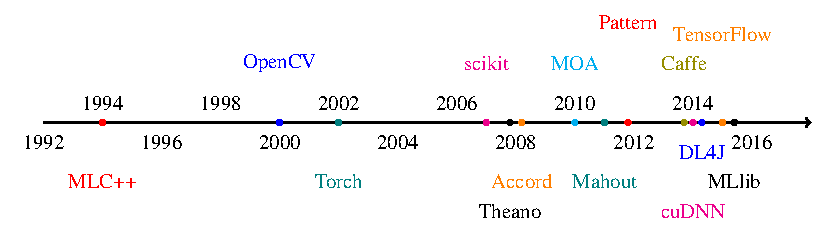
\includegraphics[width=0.9\linewidth]{figures/ML.pdf} 
\end{figure}

\begin{center}
{\color{red} \scriptsize
Tour of TensorFlow, by Peter Goldsborough, arXiv, 2016}
\end{center}


\end{frame}

%%%
\subsection{DL code}
%%%

\begin{frame}
  \MyLogo
  \frametitle{Deep Learning: Pros and Cons}  

\small

\begin{mdframed}[style=mystyle2]
Deep Learning has been introduced with the objective of moving ML closer to one of its original goals---AI. The main motivations includes:
%
\begin{itemize}\scriptsize\setlength\itemsep{0.2em}
\item Insufficient depth can hurt
\item The brain has a deep architecture
\item Cognitive processes seem deep
\end{itemize}
\end{mdframed}

\medskip

\begin{columns}

\column{.49\textwidth}
{\color{blue}Pros:}
\begin{itemize}\setlength\itemsep{0.2em}
\item conceptually simple
\item nonlinear 
\item highly flexible and configurable
\item learned features can be extracted
\item can be fine-tuned with more data
\item efficient for multi-class problems
\item world-class at pattern recognition
\end{itemize}

\column{.51\textwidth}
{\color{red}Cons:}
\begin{itemize}\setlength\itemsep{0.2em}
\item hard to interpret 
\item theory not well understood
\item slow to train and score
\item overfits, needs regularization
\item more parameters
\item inefficient for categorical variables
\item data hungry, learns slowly 
\end{itemize}
\end{columns}

\begin{center}
{\color{red} \scriptsize
https://www.slideshare.net/0xdata/transform-your-business-with-ai-deep-learning-and-machine-learning}
\end{center}

\end{frame}

%%%
\subsection{General comparison}
%%%

\begin{frame}
  \MyLogo
  \frametitle{Popular Packages: Basic Information}  
\small

\vskip -5pt
\renewcommand{\multirowsetup}{\centering} 
\begin{table}[htdp]
\begin{center}
\begin{tabular}{|c|c|c|c|c|c|} \hline
\rowcolor{GreenYellow}
Viewpoint &Torch       &Caffe   & TensorFlow  & MXNet \\ \hline
 Started      & 2002      &2013               &2015                & 2015                    \\ \hline
 \multirow{3}{4em}{Main \\ Developers}
 & Facebook,        &\multirow{3}{5em}{BAIR}  &\multirow{3}{3em}{Google} &\multirow{3}{*}{DMLC}   \\ 
 &Twitter,            & & &    \\
 &Google, ...       & & &  \\ \hline 
 \multirow{2}{4em}{ License }     
& \multirow{2}{3em}{BSD}      
&\multirow{2}{4em}{BSD}
&\multirow{2}{4em}{Apache}
&\multirow{2}{6em}{Apache}  \\ 
&   &    & &      \\ \hline
\multirow{2}{4em}{ Core \\ Languages}     
& \multirow{2}{3em}{ C/Lua }      
&\multirow{2}{4em}{ C++}
&\multirow{2}{4em}{ C++\\Python}
&\multirow{2}{6em}{ C++}  \\ 
&   &    & &      \\ \hline
\multirow{2}{4em} {Supported \\Interface }    
& \multirow{2}{3em}{ Lua }      
&\multirow{2}{5.5em}{ C++/Python \\ Matlab}
&\multirow{2}{5.5em}{ C++/\alert{Python} \\ \alert{R}/Java/Go}  
&\multirow{2}{5.5em}{ C++/\alert{Python} \\ \alert{R}/Julia/Matlab}\\  
&   &    & &      \\ \hline           
\end{tabular}
\end{center}
\label{default}
\end{table}%

{\scriptsize
\begin{itemize}\setlength\itemsep{0.5em}
\item[\raisebox{-0.4ex}{\alert{\HandRight}}] Other worth-noting's: CNTK/DMTK (Microsoft), Neon (Nervana \& Intel), PyTorch (\alert{beta})
\item BAIR, Berkeley Artificial Intelligence Research Lab 
\item DMLC, Distributed (Deep) Machine Learning Community, supported by Amazon, Intel, Microsoft, nVidia, Baidu, ...
\end{itemize}
}

\begin{center}
{\color{red}\scriptsize
http://blog.revolutionanalytics.com/2016/08/deep-learning-part-1.html
}
\end{center}

\end{frame}

%%%

\begin{frame}
  \MyLogo
  \frametitle{Popular Packages: Performance}  
\small

\vskip -5pt
\renewcommand{\multirowsetup}{\centering} 
\begin{table}[htdp]
\begin{center}
\begin{tabular}{|c|c|c|c|c|c|} \hline
\rowcolor{GreenYellow}
Viewpoint &Torch       &Caffe  & TensorFlow & MXNet  \\ \hline
  \multirow{2}{4em}{Pretrained \\ Models}      
  &  \multirow{2}{4em} {Yes}      
  &  \multirow{2}{4em}{Yes}                             
  &  \multirow{2}{4em}{No}                   
  &  \multirow{2}{4em}{Yes}\\ 
  &  &   &   & \\ \hline
\multirow{2}{4.5em}{High-level \\ Support}     
& \multirow{2}{*}{Good}      
&\multirow{2}{*}{ Good}
&\multirow{2}{*}{ Good}
&\multirow{2}{*}{ Good}  \\ 
&   &    & &      \\ \hline
 \multirow{2}{4em}{Low-level \\ Operators}
 &\multirow{2}{4em}{Good}
 &\multirow{2}{*}{Good }     
 &\multirow{2}{*}{Fairly good}
 &\multirow{2}{*}{Very few}\\ 
 &       &    &  &  \\ \hline 
\multirow{2}{4em} {Speed \\ One-GPU }    
& \multirow{2}{*}{ Great }      
&\multirow{2}{*}{Great} 
&\multirow{2}{*}{\alert{Not so good}}
&\multirow{2}{*}{ Excellent} \\  
&   &    & &      \\ \hline          
\multirow{2}{5em} {Memory \\ Management}    
& \multirow{2}{*}{ Great }      
&\multirow{2}{*}{Great}
&\multirow{2}{*}{\alert{Not so good}}
&\multirow{2}{*}{ Excellent}  \\  
&   &    & &      \\ \hline            
\multirow{2}{3.5em} {Parallel \\ Support}    
& \multirow{2}{5.em}{Multi-GPU}      
&\multirow{2}{5.em}{Multi-GPU}
&\multirow{2}{5.em}{Multi-GPU} 
&\multirow{2}{5em}{Distributed} \\  
&   &    & &      \\ \hline            
\multirow{2}{3.5em} {Coding \\ Style}    
& \multirow{2}{5.em}{Imperative}      
&\multirow{2}{5.em}{Imperative}
&\multirow{2}{5.em}{Declarative} 
&\multirow{2}{5em}{Declarative \\ Imperative} \\  
&   &    & &      \\ \hline
\multirow{2}{3.5em} {GitHub \\ Watching}    
& \multirow{2}{5.em}{649/268}      
&\multirow{2}{5.em}{1856}
&\multirow{2}{5.em}{4939} 
&\multirow{2}{5em}{887} \\  
&   &    & &      \\ \hline
\end{tabular}
\end{center}
\label{default}
\end{table}%

\end{frame}
